\documentclass{whiteboard}
\begin{document}
\begin{frame}[plain,t]
 \bbcover{CSES 1673}{High Score}{Prof. Edson Alves}{Faculdade UnB Gama}
\end{frame}

\begin{frame}[plain,t]
\vspace*{\fill}
 \bbenglish{You play a game consisting of $n$ rooms and $m$ tunnels. Your initial score is $0$, and each tunnel increases your score by $x$ where $x$ may be both positive or negative. You may go through a tunnel several times.}

 \vspace{0.1in}

 \bbenglish{Your task is to walk from room $1$ to room $n$. What is the maximum score you can get?}
\vspace*{\fill}
\end{frame}

\begin{frame}[plain,t]
\vspace*{\fill}
 \bbtext{Você vai jogar um jogo composto por $n$ salas e $m$ túneis. Sua pontuação inicial é igual a $0$, e cada túnel aumenta sua pontuação em $x$ unidades, onde $x$ pode ser tanto positivo quanto negativo. Você pode passar por um mesmo túnel várias vezes.}

 \vspace{0.1in}

 \bbtext{Sua tarefa é ir da sala $1$ para a sala $n$. Qual é a maior pontuação que você pode obter?}
\vspace*{\fill}
\end{frame}

\begin{frame}[plain,t]
\vspace*{\fill}
 \bbbold{Input}

 \vspace{0.1in}

 \bbenglish{The first input line has two integers $n$ and $m$: the number of rooms and tunnels. The rooms are numbered $1, 2, \ldots , n$.}

 \vspace{0.1in}

 \bbenglish{Then, there are m lines describing the tunnels. Each line has three integers $a, b$ and $x$: the tunnel starts at room $a$, ends at room $b$, and it increases your score by $x$. All tunnels are one-way tunnels.}

 \vspace{0.1in}

 \bbenglish{You can assume that it is possible to get from room $1$ to room $n$.}

 \vspace{0.2in}

 \bbbold{Output}

 \vspace{0.1in}

 \bbenglish{Print one integer: the maximum score you can get. However, if you can get an arbitrarily large score, print $-1$.}
\vspace*{\fill}
\end{frame}

\begin{frame}[plain,t]
\vspace*{\fill}
 \bbbold{Entrada}

 \vspace{0.1in}

 \bbtext{A primeira linha da entrada contém dois inteiros $n$ e $m$: o número de salas e de túneis. As salas são numeradas $1, 2, \ldots , n$.}

 \vspace{0.1in}

 \bbtext{As $m$ linhas seguintes descrevem os túneis. Cada linha tem três inteiros $a, b$ e $x$: o túnel começa na sala $a$, termina na sala $b$ e aumenta sua pontuação em $x$ unidades. Todos os túneis são de mão única.}

 \vspace{0.1in}

 \bbtext{Assuma que é possível ir da sala $1$ para a sala $n$.}

 \vspace{0.2in}

 \bbbold{Saída}

 \vspace{0.1in}

 \bbtext{Imprima um inteiro: a pontuação máxima que você pode obter. Contudo, se você pode obter uma pontuação arbitrariamente grande, imprima $-1$.}
\vspace*{\fill}
\end{frame}

\begin{frame}[plain,t]
\vspace*{\fill}
 \bbbold{Constraints}

 \vspace{0.1in}

 \begin{itemize} \item $1\leq 2500\leq n$ \item $1\leq 5000\leq m$ \item $1\leq a, b\leq n$ \item $-10^9 \leq x\leq 10^9$\end{itemize}
\vspace*{\fill}
\end{frame}

\begin{frame}[plain,t]
\vspace*{\fill}
 \bbbold{Restrições}

 \vspace{0.1in}

 \begin{itemize} \item $1\leq 2500\leq n$ \item $1\leq 5000\leq m$ \item $1\leq a, b\leq n$ \item $-10^9 \leq x\leq 10^9$\end{itemize}
\vspace*{\fill}
\end{frame}

\begin{frame}[plain,t]
\begin{tikzpicture}
\node[draw,opacity=0] at (0, 0) {x};
\node[draw,opacity=0] at (14, 8) {x};
 \node[anchor=west] at (0, 7) { \bbbold{Exemplo de entrada e saída} };
\end{tikzpicture}
\end{frame}

\begin{frame}[plain,t]
\begin{tikzpicture}
\node[draw,opacity=0] at (0, 0) {x};
\node[draw,opacity=0] at (14, 8) {x};
 \node[anchor=west] at (0, 7) { \bbbold{Exemplo de entrada e saída} };
 \node[anchor=west] at (1, 6) { \bbtext{4 5} };
\end{tikzpicture}
\end{frame}

\begin{frame}[plain,t]
\begin{tikzpicture}
\node[draw,opacity=0] at (0, 0) {x};
\node[draw,opacity=0] at (14, 8) {x};
 \node[anchor=west] at (0, 7) { \bbbold{Exemplo de entrada e saída} };
 \node[anchor=west] at (1, 6) { \bbtext{4 5} };
 \node at (1.25, 5) { \footnotesize \bbcomment{\# de salas} };
 \draw[->,color=BBViolet] (1.25, 5.2) -- (1.25, 5.8);
\end{tikzpicture}
\end{frame}

\begin{frame}[plain,t]
\begin{tikzpicture}
\node[draw,opacity=0] at (0, 0) {x};
\node[draw,opacity=0] at (14, 8) {x};
 \node[anchor=west] at (0, 7) { \bbbold{Exemplo de entrada e saída} };
 \node[anchor=west] at (1, 6) { \bbtext{4 5} };
 \node at (1.25, 5) { \footnotesize \bbcomment{\# de salas} };
 \draw[->,color=BBViolet] (1.25, 5.2) -- (1.25, 5.8);
 \node[draw,very thick,circle] (A) at (6, 4) { \bbtext{1} };
 \node[draw,very thick,circle] (B) at (9, 7) { \bbtext{2} };
 \node[draw,very thick,circle] (C) at (12, 4) { \bbtext{3} };
 \node[draw,very thick,circle] (D) at (9, 1) { \bbtext{4} };
\end{tikzpicture}
\end{frame}

\begin{frame}[plain,t]
\begin{tikzpicture}
\node[draw,opacity=0] at (0, 0) {x};
\node[draw,opacity=0] at (14, 8) {x};
 \node[anchor=west] at (0, 7) { \bbbold{Exemplo de entrada e saída} };
 \node[anchor=west] at (1, 6) { \bbtext{4 5} };
 \node at (1.25, 5) { \footnotesize \bbcomment{\# de salas} };
 \draw[->,color=BBViolet] (1.25, 5.2) -- (1.25, 5.8);
 \node[draw,very thick,circle] (A) at (6, 4) { \bbtext{1} };
 \node[draw,very thick,circle] (B) at (9, 7) { \bbtext{2} };
 \node[draw,very thick,circle] (C) at (12, 4) { \bbtext{3} };
 \node[draw,very thick,circle] (D) at (9, 1) { \bbtext{4} };
 \node[anchor=west] at (2.75, 6) { \footnotesize \bbcomment{\# de túneis} };
 \draw[->,color=BBViolet] (1.75, 6) -- (2.75, 6);
\end{tikzpicture}
\end{frame}

\begin{frame}[plain,t]
\begin{tikzpicture}
\node[draw,opacity=0] at (0, 0) {x};
\node[draw,opacity=0] at (14, 8) {x};
 \node[anchor=west] at (0, 7) { \bbbold{Exemplo de entrada e saída} };
 \node[anchor=west] at (1, 6) { \bbtext{4 5} };
 \node[draw,very thick,circle] (A) at (6, 4) { \bbtext{1} };
 \node[draw,very thick,circle] (B) at (9, 7) { \bbtext{2} };
 \node[draw,very thick,circle] (C) at (12, 4) { \bbtext{3} };
 \node[draw,very thick,circle] (D) at (9, 1) { \bbtext{4} };
\end{tikzpicture}
\end{frame}

\begin{frame}[plain,t]
\begin{tikzpicture}
\node[draw,opacity=0] at (0, 0) {x};
\node[draw,opacity=0] at (14, 8) {x};
 \node[anchor=west] at (0, 7) { \bbbold{Exemplo de entrada e saída} };
 \node[anchor=west] at (1, 6) { \bbtext{4 5} };
 \node[draw,very thick,circle] (A) at (6, 4) { \bbtext{1} };
 \node[draw,very thick,circle] (B) at (9, 7) { \bbtext{2} };
 \node[draw,very thick,circle] (C) at (12, 4) { \bbtext{3} };
 \node[draw,very thick,circle] (D) at (9, 1) { \bbtext{4} };
 \node[anchor=west] at (1, 5) { \bbtext{1 2 3} };
\end{tikzpicture}
\end{frame}

\begin{frame}[plain,t]
\begin{tikzpicture}
\node[draw,opacity=0] at (0, 0) {x};
\node[draw,opacity=0] at (14, 8) {x};
 \node[anchor=west] at (0, 7) { \bbbold{Exemplo de entrada e saída} };
 \node[anchor=west] at (1, 6) { \bbtext{4 5} };
 \node[draw,very thick,circle] (A) at (6, 4) { \bbtext{1} };
 \node[draw,very thick,circle] (B) at (9, 7) { \bbtext{2} };
 \node[draw,very thick,circle] (C) at (12, 4) { \bbtext{3} };
 \node[draw,very thick,circle] (D) at (9, 1) { \bbtext{4} };
 \node[anchor=west] at (1, 5) { \bbtext{1 2 3} };
 \node at (1.25, 4) { \footnotesize $a$ };
 \draw[->,color=BBViolet] (1.25, 4.2) -- (1.25, 4.8);
\end{tikzpicture}
\end{frame}

\begin{frame}[plain,t]
\begin{tikzpicture}
\node[draw,opacity=0] at (0, 0) {x};
\node[draw,opacity=0] at (14, 8) {x};
 \node[anchor=west] at (0, 7) { \bbbold{Exemplo de entrada e saída} };
 \node[anchor=west] at (1, 6) { \bbtext{4 5} };
 \node[draw,very thick,circle] (A) at (6, 4) { \bbtext{1} };
 \node[draw,very thick,circle] (B) at (9, 7) { \bbtext{2} };
 \node[draw,very thick,circle] (C) at (12, 4) { \bbtext{3} };
 \node[draw,very thick,circle] (D) at (9, 1) { \bbtext{4} };
 \node[anchor=west] at (1, 5) { \bbtext{1 2 3} };
 \node at (1.25, 4) { \footnotesize $a$ };
 \draw[->,color=BBViolet] (1.25, 4.2) -- (1.25, 4.8);
 \node at (1.55, 4) { \footnotesize $b$ };
 \draw[->,color=BBViolet] (1.55, 4.2) -- (1.55, 4.8);
\end{tikzpicture}
\end{frame}

\begin{frame}[plain,t]
\begin{tikzpicture}
\node[draw,opacity=0] at (0, 0) {x};
\node[draw,opacity=0] at (14, 8) {x};
 \node[anchor=west] at (0, 7) { \bbbold{Exemplo de entrada e saída} };
 \node[anchor=west] at (1, 6) { \bbtext{4 5} };
 \node[draw,very thick,circle] (A) at (6, 4) { \bbtext{1} };
 \node[draw,very thick,circle] (B) at (9, 7) { \bbtext{2} };
 \node[draw,very thick,circle] (C) at (12, 4) { \bbtext{3} };
 \node[draw,very thick,circle] (D) at (9, 1) { \bbtext{4} };
 \node[anchor=west] at (1, 5) { \bbtext{1 2 3} };
 \node at (1.25, 4) { \footnotesize $a$ };
 \draw[->,color=BBViolet] (1.25, 4.2) -- (1.25, 4.8);
 \node at (1.55, 4) { \footnotesize $b$ };
 \draw[->,color=BBViolet] (1.55, 4.2) -- (1.55, 4.8);
 \node at (1.88, 4) { \footnotesize $x$ };
 \draw[->,color=BBViolet] (1.88, 4.2) -- (1.88, 4.8);
\end{tikzpicture}
\end{frame}

\begin{frame}[plain,t]
\begin{tikzpicture}
\node[draw,opacity=0] at (0, 0) {x};
\node[draw,opacity=0] at (14, 8) {x};
 \node[anchor=west] at (0, 7) { \bbbold{Exemplo de entrada e saída} };
 \node[anchor=west] at (1, 6) { \bbtext{4 5} };
 \node[draw,very thick,circle] (A) at (6, 4) { \bbtext{1} };
 \node[draw,very thick,circle] (B) at (9, 7) { \bbtext{2} };
 \node[draw,very thick,circle] (C) at (12, 4) { \bbtext{3} };
 \node[draw,very thick,circle] (D) at (9, 1) { \bbtext{4} };
 \node[anchor=west] at (1, 5) { \bbtext{1 2 3} };
 \draw[-latex,thick] (A) to node[above] { \bbinfo{3} } (B);
\end{tikzpicture}
\end{frame}

\begin{frame}[plain,t]
\begin{tikzpicture}
\node[draw,opacity=0] at (0, 0) {x};
\node[draw,opacity=0] at (14, 8) {x};
 \node[anchor=west] at (0, 7) { \bbbold{Exemplo de entrada e saída} };
 \node[anchor=west] at (1, 6) { \bbtext{4 5} };
 \node[draw,very thick,circle] (A) at (6, 4) { \bbtext{1} };
 \node[draw,very thick,circle] (B) at (9, 7) { \bbtext{2} };
 \node[draw,very thick,circle] (C) at (12, 4) { \bbtext{3} };
 \node[draw,very thick,circle] (D) at (9, 1) { \bbtext{4} };
 \node[anchor=west] at (1, 5) { \bbtext{1 2 3} };
 \draw[-latex,thick] (A) to node[above] { \bbinfo{3} } (B);
 \node[anchor=west] at (1, 4.5) { \bbtext{2 4 -1} };
\end{tikzpicture}
\end{frame}

\begin{frame}[plain,t]
\begin{tikzpicture}
\node[draw,opacity=0] at (0, 0) {x};
\node[draw,opacity=0] at (14, 8) {x};
 \node[anchor=west] at (0, 7) { \bbbold{Exemplo de entrada e saída} };
 \node[anchor=west] at (1, 6) { \bbtext{4 5} };
 \node[draw,very thick,circle] (A) at (6, 4) { \bbtext{1} };
 \node[draw,very thick,circle] (B) at (9, 7) { \bbtext{2} };
 \node[draw,very thick,circle] (C) at (12, 4) { \bbtext{3} };
 \node[draw,very thick,circle] (D) at (9, 1) { \bbtext{4} };
 \node[anchor=west] at (1, 5) { \bbtext{1 2 3} };
 \draw[-latex,thick] (A) to node[above] { \bbinfo{3} } (B);
 \node[anchor=west] at (1, 4.5) { \bbtext{2 4 -1} };
 \draw[-latex,thick] (B) to node[right,pos=0.3] { \bbinfo{-1} } (D);
\end{tikzpicture}
\end{frame}

\begin{frame}[plain,t]
\begin{tikzpicture}
\node[draw,opacity=0] at (0, 0) {x};
\node[draw,opacity=0] at (14, 8) {x};
 \node[anchor=west] at (0, 7) { \bbbold{Exemplo de entrada e saída} };
 \node[anchor=west] at (1, 6) { \bbtext{4 5} };
 \node[draw,very thick,circle] (A) at (6, 4) { \bbtext{1} };
 \node[draw,very thick,circle] (B) at (9, 7) { \bbtext{2} };
 \node[draw,very thick,circle] (C) at (12, 4) { \bbtext{3} };
 \node[draw,very thick,circle] (D) at (9, 1) { \bbtext{4} };
 \node[anchor=west] at (1, 5) { \bbtext{1 2 3} };
 \draw[-latex,thick] (A) to node[above] { \bbinfo{3} } (B);
 \node[anchor=west] at (1, 4.5) { \bbtext{2 4 -1} };
 \draw[-latex,thick] (B) to node[right,pos=0.3] { \bbinfo{-1} } (D);
 \node[anchor=west] at (1, 4.0) { \bbtext{1 3 -2} };
\end{tikzpicture}
\end{frame}

\begin{frame}[plain,t]
\begin{tikzpicture}
\node[draw,opacity=0] at (0, 0) {x};
\node[draw,opacity=0] at (14, 8) {x};
 \node[anchor=west] at (0, 7) { \bbbold{Exemplo de entrada e saída} };
 \node[anchor=west] at (1, 6) { \bbtext{4 5} };
 \node[draw,very thick,circle] (A) at (6, 4) { \bbtext{1} };
 \node[draw,very thick,circle] (B) at (9, 7) { \bbtext{2} };
 \node[draw,very thick,circle] (C) at (12, 4) { \bbtext{3} };
 \node[draw,very thick,circle] (D) at (9, 1) { \bbtext{4} };
 \node[anchor=west] at (1, 5) { \bbtext{1 2 3} };
 \draw[-latex,thick] (A) to node[above] { \bbinfo{3} } (B);
 \node[anchor=west] at (1, 4.5) { \bbtext{2 4 -1} };
 \draw[-latex,thick] (B) to node[right,pos=0.3] { \bbinfo{-1} } (D);
 \node[anchor=west] at (1, 4.0) { \bbtext{1 3 -2} };
 \draw[-latex,thick] (A) to node[above,pos=0.3] { \bbinfo{-2} } (C);
\end{tikzpicture}
\end{frame}

\begin{frame}[plain,t]
\begin{tikzpicture}
\node[draw,opacity=0] at (0, 0) {x};
\node[draw,opacity=0] at (14, 8) {x};
 \node[anchor=west] at (0, 7) { \bbbold{Exemplo de entrada e saída} };
 \node[anchor=west] at (1, 6) { \bbtext{4 5} };
 \node[draw,very thick,circle] (A) at (6, 4) { \bbtext{1} };
 \node[draw,very thick,circle] (B) at (9, 7) { \bbtext{2} };
 \node[draw,very thick,circle] (C) at (12, 4) { \bbtext{3} };
 \node[draw,very thick,circle] (D) at (9, 1) { \bbtext{4} };
 \node[anchor=west] at (1, 5) { \bbtext{1 2 3} };
 \draw[-latex,thick] (A) to node[above] { \bbinfo{3} } (B);
 \node[anchor=west] at (1, 4.5) { \bbtext{2 4 -1} };
 \draw[-latex,thick] (B) to node[right,pos=0.3] { \bbinfo{-1} } (D);
 \node[anchor=west] at (1, 4.0) { \bbtext{1 3 -2} };
 \draw[-latex,thick] (A) to node[above,pos=0.3] { \bbinfo{-2} } (C);
 \node[anchor=west] at (1, 3.5) { \bbtext{3 4 7} };
\end{tikzpicture}
\end{frame}

\begin{frame}[plain,t]
\begin{tikzpicture}
\node[draw,opacity=0] at (0, 0) {x};
\node[draw,opacity=0] at (14, 8) {x};
 \node[anchor=west] at (0, 7) { \bbbold{Exemplo de entrada e saída} };
 \node[anchor=west] at (1, 6) { \bbtext{4 5} };
 \node[draw,very thick,circle] (A) at (6, 4) { \bbtext{1} };
 \node[draw,very thick,circle] (B) at (9, 7) { \bbtext{2} };
 \node[draw,very thick,circle] (C) at (12, 4) { \bbtext{3} };
 \node[draw,very thick,circle] (D) at (9, 1) { \bbtext{4} };
 \node[anchor=west] at (1, 5) { \bbtext{1 2 3} };
 \draw[-latex,thick] (A) to node[above] { \bbinfo{3} } (B);
 \node[anchor=west] at (1, 4.5) { \bbtext{2 4 -1} };
 \draw[-latex,thick] (B) to node[right,pos=0.3] { \bbinfo{-1} } (D);
 \node[anchor=west] at (1, 4.0) { \bbtext{1 3 -2} };
 \draw[-latex,thick] (A) to node[above,pos=0.3] { \bbinfo{-2} } (C);
 \node[anchor=west] at (1, 3.5) { \bbtext{3 4 7} };
 \draw[-latex,thick] (C) to node[above] { \bbinfo{7} } (D);
\end{tikzpicture}
\end{frame}

\begin{frame}[plain,t]
\begin{tikzpicture}
\node[draw,opacity=0] at (0, 0) {x};
\node[draw,opacity=0] at (14, 8) {x};
 \node[anchor=west] at (0, 7) { \bbbold{Exemplo de entrada e saída} };
 \node[anchor=west] at (1, 6) { \bbtext{4 5} };
 \node[draw,very thick,circle] (A) at (6, 4) { \bbtext{1} };
 \node[draw,very thick,circle] (B) at (9, 7) { \bbtext{2} };
 \node[draw,very thick,circle] (C) at (12, 4) { \bbtext{3} };
 \node[draw,very thick,circle] (D) at (9, 1) { \bbtext{4} };
 \node[anchor=west] at (1, 5) { \bbtext{1 2 3} };
 \draw[-latex,thick] (A) to node[above] { \bbinfo{3} } (B);
 \node[anchor=west] at (1, 4.5) { \bbtext{2 4 -1} };
 \draw[-latex,thick] (B) to node[right,pos=0.3] { \bbinfo{-1} } (D);
 \node[anchor=west] at (1, 4.0) { \bbtext{1 3 -2} };
 \draw[-latex,thick] (A) to node[above,pos=0.3] { \bbinfo{-2} } (C);
 \node[anchor=west] at (1, 3.5) { \bbtext{3 4 7} };
 \draw[-latex,thick] (C) to node[above] { \bbinfo{7} } (D);
 \node[anchor=west] at (1, 3.0) { \bbtext{1 4 4} };
\end{tikzpicture}
\end{frame}

\begin{frame}[plain,t]
\begin{tikzpicture}
\node[draw,opacity=0] at (0, 0) {x};
\node[draw,opacity=0] at (14, 8) {x};
 \node[anchor=west] at (0, 7) { \bbbold{Exemplo de entrada e saída} };
 \node[anchor=west] at (1, 6) { \bbtext{4 5} };
 \node[draw,very thick,circle] (A) at (6, 4) { \bbtext{1} };
 \node[draw,very thick,circle] (B) at (9, 7) { \bbtext{2} };
 \node[draw,very thick,circle] (C) at (12, 4) { \bbtext{3} };
 \node[draw,very thick,circle] (D) at (9, 1) { \bbtext{4} };
 \node[anchor=west] at (1, 5) { \bbtext{1 2 3} };
 \draw[-latex,thick] (A) to node[above] { \bbinfo{3} } (B);
 \node[anchor=west] at (1, 4.5) { \bbtext{2 4 -1} };
 \draw[-latex,thick] (B) to node[right,pos=0.3] { \bbinfo{-1} } (D);
 \node[anchor=west] at (1, 4.0) { \bbtext{1 3 -2} };
 \draw[-latex,thick] (A) to node[above,pos=0.3] { \bbinfo{-2} } (C);
 \node[anchor=west] at (1, 3.5) { \bbtext{3 4 7} };
 \draw[-latex,thick] (C) to node[above] { \bbinfo{7} } (D);
 \node[anchor=west] at (1, 3.0) { \bbtext{1 4 4} };
 \draw[-latex,thick] (A) to node[above] { \bbinfo{4} } (D);
\end{tikzpicture}
\end{frame}

\begin{frame}[plain,t]
\begin{tikzpicture}
\node[draw,opacity=0] at (0, 0) {x};
\node[draw,opacity=0] at (14, 8) {x};
 \node[anchor=west] at (0, 7) { \bbbold{Exemplo de entrada e saída} };
 \node[anchor=west] at (1, 6) { \bbtext{4 5} };
 \node[draw,very thick,circle] (A) at (6, 4) { \bbtext{1} };
 \node[draw,very thick,circle] (B) at (9, 7) { \bbtext{2} };
 \node[draw,very thick,circle] (C) at (12, 4) { \bbtext{3} };
 \node[draw,very thick,circle] (D) at (9, 1) { \bbtext{4} };
 \node[anchor=west] at (1, 5) { \bbtext{1 2 3} };
 \node[anchor=west] at (1, 4.5) { \bbtext{2 4 -1} };
 \node[anchor=west] at (1, 4.0) { \bbtext{1 3 -2} };
 \draw[-latex,thick] (A) to node[above,pos=0.3] { \bbinfo{-2} } (C);
 \node[anchor=west] at (1, 3.5) { \bbtext{3 4 7} };
 \draw[-latex,thick] (C) to node[above] { \bbinfo{7} } (D);
 \node[anchor=west] at (1, 3.0) { \bbtext{1 4 4} };
 \draw[-latex,thick] (A) to node[above] { \bbinfo{4} } (D);
 \draw[-latex,very thick,color=BBRed,dashed] (1, 2) to (2.0, 2);
 \node[anchor=west] at (2.0, 2) { $3 - 1 = 2$ };
 \draw[-latex,very thick,color=BBRed,dashed] (A) to node[above] { \bbinfo{3} } (B);
 \draw[-latex,very thick,color=BBRed,dashed] (B) to node[right,pos=0.3] { \bbinfo{-1} } (D);
\end{tikzpicture}
\end{frame}

\begin{frame}[plain,t]
\begin{tikzpicture}
\node[draw,opacity=0] at (0, 0) {x};
\node[draw,opacity=0] at (14, 8) {x};
 \node[anchor=west] at (0, 7) { \bbbold{Exemplo de entrada e saída} };
 \node[anchor=west] at (1, 6) { \bbtext{4 5} };
 \node[draw,very thick,circle] (A) at (6, 4) { \bbtext{1} };
 \node[draw,very thick,circle] (B) at (9, 7) { \bbtext{2} };
 \node[draw,very thick,circle] (C) at (12, 4) { \bbtext{3} };
 \node[draw,very thick,circle] (D) at (9, 1) { \bbtext{4} };
 \node[anchor=west] at (1, 5) { \bbtext{1 2 3} };
 \node[anchor=west] at (1, 4.5) { \bbtext{2 4 -1} };
 \node[anchor=west] at (1, 4.0) { \bbtext{1 3 -2} };
 \draw[-latex,thick] (A) to node[above,pos=0.3] { \bbinfo{-2} } (C);
 \node[anchor=west] at (1, 3.5) { \bbtext{3 4 7} };
 \draw[-latex,thick] (C) to node[above] { \bbinfo{7} } (D);
 \node[anchor=west] at (1, 3.0) { \bbtext{1 4 4} };
 \draw[-latex,very thick,color=BBRed,dashed] (1, 2) to (2.0, 2);
 \node[anchor=west] at (2.0, 2) { $3 - 1 = 2$ };
 \draw[-latex,very thick,color=BBRed,dashed] (A) to node[above] { \bbinfo{3} } (B);
 \draw[-latex,very thick,color=BBRed,dashed] (B) to node[right,pos=0.3] { \bbinfo{-1} } (D);
 \draw[-latex,very thick,color=BBViolet,dashed] (1, 1.5) to (2.0, 1.5);
 \node[anchor=west] at (2.0, 1.5) { $4$ };
 \draw[-latex,very thick,color=BBViolet,dashed] (A) to node[above] { \bbinfo{4} } (D);
\end{tikzpicture}
\end{frame}

\begin{frame}[plain,t]
\begin{tikzpicture}
\node[draw,opacity=0] at (0, 0) {x};
\node[draw,opacity=0] at (14, 8) {x};
 \node[anchor=west] at (0, 7) { \bbbold{Exemplo de entrada e saída} };
 \node[anchor=west] at (1, 6) { \bbtext{4 5} };
 \node[draw,very thick,circle] (A) at (6, 4) { \bbtext{1} };
 \node[draw,very thick,circle] (B) at (9, 7) { \bbtext{2} };
 \node[draw,very thick,circle] (C) at (12, 4) { \bbtext{3} };
 \node[draw,very thick,circle] (D) at (9, 1) { \bbtext{4} };
 \node[anchor=west] at (1, 5) { \bbtext{1 2 3} };
 \node[anchor=west] at (1, 4.5) { \bbtext{2 4 -1} };
 \node[anchor=west] at (1, 4.0) { \bbtext{1 3 -2} };
 \node[anchor=west] at (1, 3.5) { \bbtext{3 4 7} };
 \node[anchor=west] at (1, 3.0) { \bbtext{1 4 4} };
 \draw[-latex,very thick,color=BBRed,dashed] (1, 2) to (2.0, 2);
 \node[anchor=west] at (2.0, 2) { $3 - 1 = 2$ };
 \draw[-latex,very thick,color=BBRed,dashed] (A) to node[above] { \bbinfo{3} } (B);
 \draw[-latex,very thick,color=BBRed,dashed] (B) to node[right,pos=0.3] { \bbinfo{-1} } (D);
 \draw[-latex,very thick,color=BBViolet,dashed] (1, 1.5) to (2.0, 1.5);
 \node[anchor=west] at (2.0, 1.5) { $4$ };
 \draw[-latex,very thick,color=BBViolet,dashed] (A) to node[above] { \bbinfo{4} } (D);
 \draw[-latex,very thick,color=BBGreen] (1, 1.0) to (2.0, 1.0);
 \node[anchor=west] at (2.0, 1.0) { $7 - 2 = 5$ };
 \draw[-latex,very thick,color=BBGreen] (A) to node[above,pos=0.3] { \bbinfo{-2} } (C);
 \draw[-latex,very thick,color=BBGreen] (C) to node[above] { \bbinfo{7} } (D);
\end{tikzpicture}
\end{frame}

\begin{frame}[plain,t]
\begin{tikzpicture}
\node[draw,opacity=0] at (0, 0) {x};
\node[draw,opacity=0] at (14, 8) {x};
 \node[anchor=west] at (0, 7) { \Large \bbbold{Solução} };
\end{tikzpicture}
\end{frame}

\begin{frame}[plain,t]
\begin{tikzpicture}
\node[draw,opacity=0] at (0, 0) {x};
\node[draw,opacity=0] at (14, 8) {x};
 \node[anchor=west] at (0, 7) { \Large \bbbold{Solução} };
 \node[anchor=west] at (1, 6) { \bbtext{Como computar o caminho máximo usando Bellman-Ford?} };
\end{tikzpicture}
\end{frame}

\begin{frame}[plain,t]
\begin{tikzpicture}
\node[draw,opacity=0] at (0, 0) {x};
\node[draw,opacity=0] at (14, 8) {x};
 \node[anchor=west] at (0, 7) { \Large \bbbold{Solução} };
 \node[anchor=west] at (1, 6) { \bbtext{Como computar o caminho máximo usando Bellman-Ford?} };
 \node[anchor=west] at (1.5, 5) { \bbcomment{Inverta o sinal das arestas e compute o caminho mínimo!} };
\end{tikzpicture}
\end{frame}

\begin{frame}[plain,t]
\begin{tikzpicture}
\node[draw,opacity=0] at (0, 0) {x};
\node[draw,opacity=0] at (14, 8) {x};
 \node[anchor=west] at (0, 7) { \Large \bbbold{Solução} };
 \node[anchor=west] at (1, 6) { \bbtext{Como computar o caminho máximo usando Bellman-Ford?} };
 \node[anchor=west] at (1.5, 5) { \bbcomment{Inverta o sinal das arestas e compute o caminho mínimo!} };
 \node[draw,very thick,circle] (A) at (1, 3) { \bbtext{A} };
 \node[draw,very thick,circle] (B) at (3, 1) { \bbtext{B} };
 \node[draw,very thick,circle] (C) at (5, 3) { \bbtext{C} };
 \draw[-latex,very thick,dashed,color=BBCyan] (A) to node[above] { \textcolor{BBOrange}{4} } (C);
 \draw[-latex,thick] (A) to node[below left] { \textcolor{BBOrange}{2} } (B);
 \draw[-latex,thick] (B) to node[below right] { \textcolor{BBOrange}{3} } (C);
\end{tikzpicture}
\end{frame}

\begin{frame}[plain,t]
\begin{tikzpicture}
\node[draw,opacity=0] at (0, 0) {x};
\node[draw,opacity=0] at (14, 8) {x};
 \node[anchor=west] at (0, 7) { \Large \bbbold{Solução} };
 \node[anchor=west] at (1, 6) { \bbtext{Como computar o caminho máximo usando Bellman-Ford?} };
 \node[anchor=west] at (1.5, 5) { \bbcomment{Inverta o sinal das arestas e compute o caminho mínimo!} };
 \node[draw,very thick,circle] (A) at (1, 3) { \bbtext{A} };
 \node[draw,very thick,circle] (B) at (3, 1) { \bbtext{B} };
 \node[draw,very thick,circle] (C) at (5, 3) { \bbtext{C} };
 \draw[-latex,very thick,dashed,color=BBCyan] (A) to node[above] { \textcolor{BBOrange}{4} } (C);
 \draw[-latex,thick] (A) to node[below left] { \textcolor{BBOrange}{2} } (B);
 \draw[-latex,thick] (B) to node[below right] { \textcolor{BBOrange}{3} } (C);
 \draw[-latex,very thick] (6, 2) to (8, 2);
\end{tikzpicture}
\end{frame}

\begin{frame}[plain,t]
\begin{tikzpicture}
\node[draw,opacity=0] at (0, 0) {x};
\node[draw,opacity=0] at (14, 8) {x};
 \node[anchor=west] at (0, 7) { \Large \bbbold{Solução} };
 \node[anchor=west] at (1, 6) { \bbtext{Como computar o caminho máximo usando Bellman-Ford?} };
 \node[anchor=west] at (1.5, 5) { \bbcomment{Inverta o sinal das arestas e compute o caminho mínimo!} };
 \node[draw,very thick,circle] (A) at (1, 3) { \bbtext{A} };
 \node[draw,very thick,circle] (B) at (3, 1) { \bbtext{B} };
 \node[draw,very thick,circle] (C) at (5, 3) { \bbtext{C} };
 \draw[-latex,very thick,dashed,color=BBCyan] (A) to node[above] { \textcolor{BBOrange}{4} } (C);
 \draw[-latex,thick] (A) to node[below left] { \textcolor{BBOrange}{2} } (B);
 \draw[-latex,thick] (B) to node[below right] { \textcolor{BBOrange}{3} } (C);
 \draw[-latex,very thick] (6, 2) to (8, 2);
 \node[draw,very thick,circle] (A) at (9, 3) { \bbtext{A} };
 \node[draw,very thick,circle] (B) at (11, 1) { \bbtext{B} };
 \node[draw,very thick,circle] (C) at (13, 3) { \bbtext{C} };
 \draw[-latex,thick] (A) to node[above] { \bbinfo{-4} } (C);
 \draw[-latex,very thick,dashed,color=BBCyan] (A) to node[below left] { \bbinfo{-2} } (B);
 \draw[-latex,very thick,dashed,color=BBCyan] (B) to node[below right] { \bbinfo{-3} } (C);
\end{tikzpicture}
\end{frame}

\begin{frame}[plain,t]
\begin{tikzpicture}
\node[draw,opacity=0] at (0, 0) {x};
\node[draw,opacity=0] at (14, 8) {x};
 \node[anchor=west] at (0, 7) { \Large \bbbold{Solução} };
\end{tikzpicture}
\end{frame}

\begin{frame}[plain,t]
\begin{tikzpicture}
\node[draw,opacity=0] at (0, 0) {x};
\node[draw,opacity=0] at (14, 8) {x};
 \node[anchor=west] at (0, 7) { \Large \bbbold{Solução} };
 \node[anchor=west] at (1, 6) { \bbtext{Como identificar ao menos um elemento de um ciclo negativo? } };
\end{tikzpicture}
\end{frame}

\begin{frame}[plain,t]
\begin{tikzpicture}
\node[draw,opacity=0] at (0, 0) {x};
\node[draw,opacity=0] at (14, 8) {x};
 \node[anchor=west] at (0, 7) { \Large \bbbold{Solução} };
 \node[anchor=west] at (1, 6) { \bbtext{Como identificar ao menos um elemento de um ciclo negativo? } };
 \node[anchor=west] at (1.5, 5) { \bbcomment{Se $\dist[u]$ é atualizado no Round \#$|V|$, então $u$ pertence a } };
 \node[anchor=west] at (3.5, 4.5) { \bbcomment{ao menos um ciclo negativo! } };
\end{tikzpicture}
\end{frame}

\begin{frame}[plain,t]
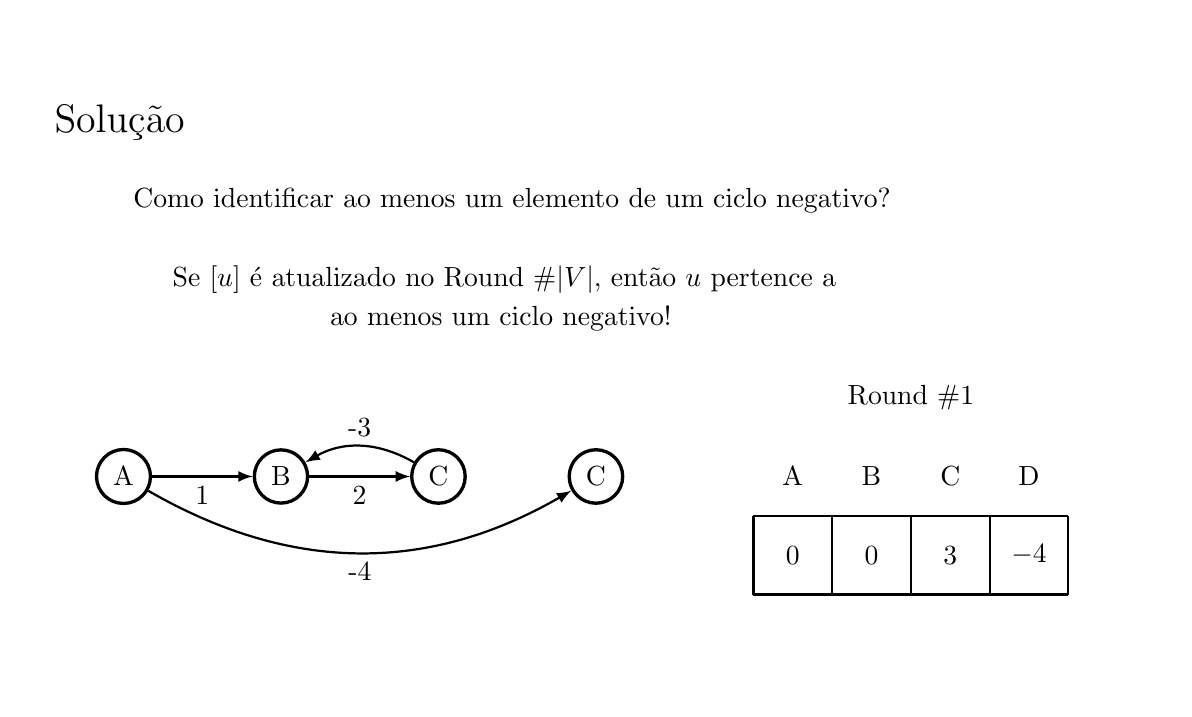
\begin{tikzpicture}
\node[draw,opacity=0] at (0, 0) {x};
\node[draw,opacity=0] at (14, 8) {x};
 \node[anchor=west] at (0, 7) { \Large \bbbold{Solução} };
 \node[anchor=west] at (1, 6) { \bbtext{Como identificar ao menos um elemento de um ciclo negativo? } };
 \node[anchor=west] at (1.5, 5) { \bbcomment{Se $\dist[u]$ é atualizado no Round \#$|V|$, então $u$ pertence a } };
 \node[anchor=west] at (3.5, 4.5) { \bbcomment{ao menos um ciclo negativo! } };
 \node[draw,very thick,circle] (A) at (1, 2.5) { \bbtext{A} };
 \node[draw,very thick,circle] (B) at (3, 2.5) { \bbtext{B} };
 \node[draw,very thick,circle] (C) at (5, 2.5) { \bbtext{C} };
 \node[draw,very thick,circle] (D) at (7, 2.5) { \bbtext{C} };
 \draw[-latex,thick] (A) to node[below] { \bbinfo{1} } (B);
 \draw[-latex,thick] (B) to node[below] { \bbinfo{2} } (C);
 \draw[-latex,thick] (C) to [bend right] node[above] { \bbinfo{-3} } (B);
 \draw[-latex,thick] (A) to [bend right] node[below] { \bbinfo{-4} } (D);
 \draw[thick] (9, 1) grid (13, 2);
 \node at (9.5, 2.5) { \bbtext{A} };
 \node at (10.5, 2.5) { \bbtext{B} };
 \node at (11.5, 2.5) { \bbtext{C} };
 \node at (12.5, 2.5) { \bbtext{D} };
 \node at (11, 3.5) { \bbbold{Round \#1} };
 \node at (9.5, 1.5) { $0$ };
 \node at (10.5, 1.5) { $0$ };
 \node at (11.5, 1.5) { $3$ };
 \node at (12.5, 1.5) { $-4$ };
\end{tikzpicture}
\end{frame}

\begin{frame}[plain,t]
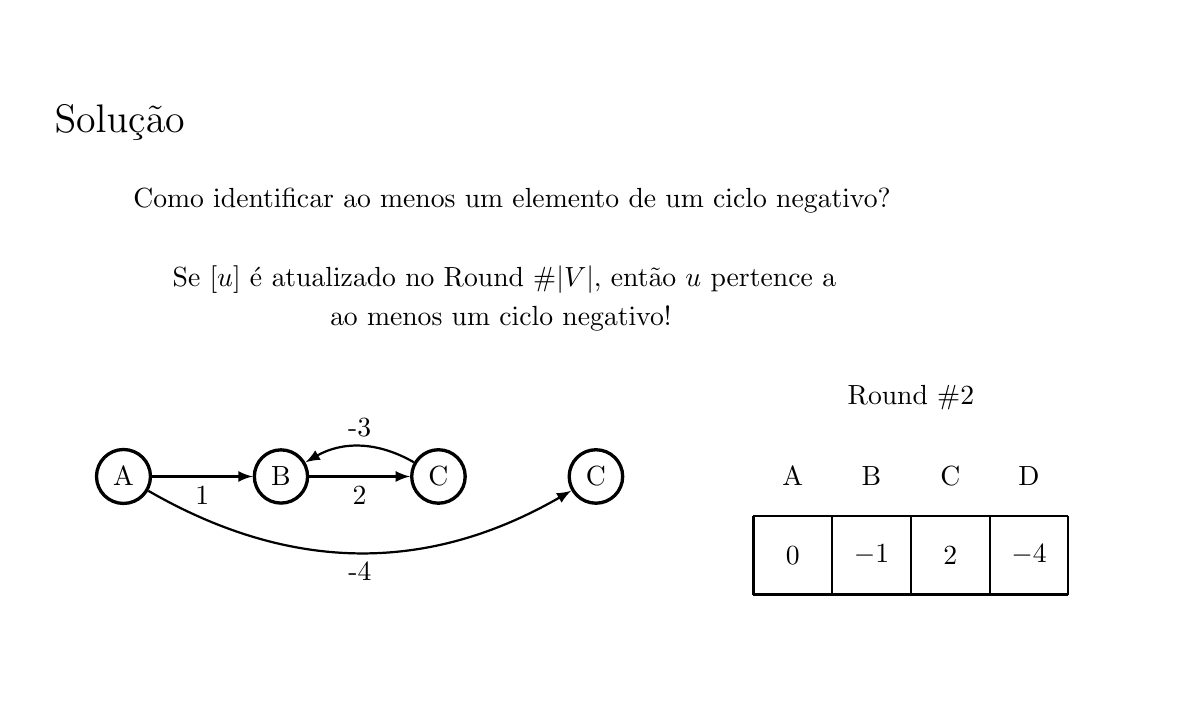
\begin{tikzpicture}
\node[draw,opacity=0] at (0, 0) {x};
\node[draw,opacity=0] at (14, 8) {x};
 \node[anchor=west] at (0, 7) { \Large \bbbold{Solução} };
 \node[anchor=west] at (1, 6) { \bbtext{Como identificar ao menos um elemento de um ciclo negativo? } };
 \node[anchor=west] at (1.5, 5) { \bbcomment{Se $\dist[u]$ é atualizado no Round \#$|V|$, então $u$ pertence a } };
 \node[anchor=west] at (3.5, 4.5) { \bbcomment{ao menos um ciclo negativo! } };
 \node[draw,very thick,circle] (A) at (1, 2.5) { \bbtext{A} };
 \node[draw,very thick,circle] (B) at (3, 2.5) { \bbtext{B} };
 \node[draw,very thick,circle] (C) at (5, 2.5) { \bbtext{C} };
 \node[draw,very thick,circle] (D) at (7, 2.5) { \bbtext{C} };
 \draw[-latex,thick] (A) to node[below] { \bbinfo{1} } (B);
 \draw[-latex,thick] (B) to node[below] { \bbinfo{2} } (C);
 \draw[-latex,thick] (C) to [bend right] node[above] { \bbinfo{-3} } (B);
 \draw[-latex,thick] (A) to [bend right] node[below] { \bbinfo{-4} } (D);
 \draw[thick] (9, 1) grid (13, 2);
 \node at (9.5, 2.5) { \bbtext{A} };
 \node at (10.5, 2.5) { \bbtext{B} };
 \node at (11.5, 2.5) { \bbtext{C} };
 \node at (12.5, 2.5) { \bbtext{D} };
 \node at (9.5, 1.5) { $0$ };
 \node at (12.5, 1.5) { $-4$ };
 \node at (11, 3.5) { \bbbold{Round \#2} };
 \node at (10.5, 1.5) { $-1$ };
 \node at (11.5, 1.5) { $2$ };
\end{tikzpicture}
\end{frame}

\begin{frame}[plain,t]
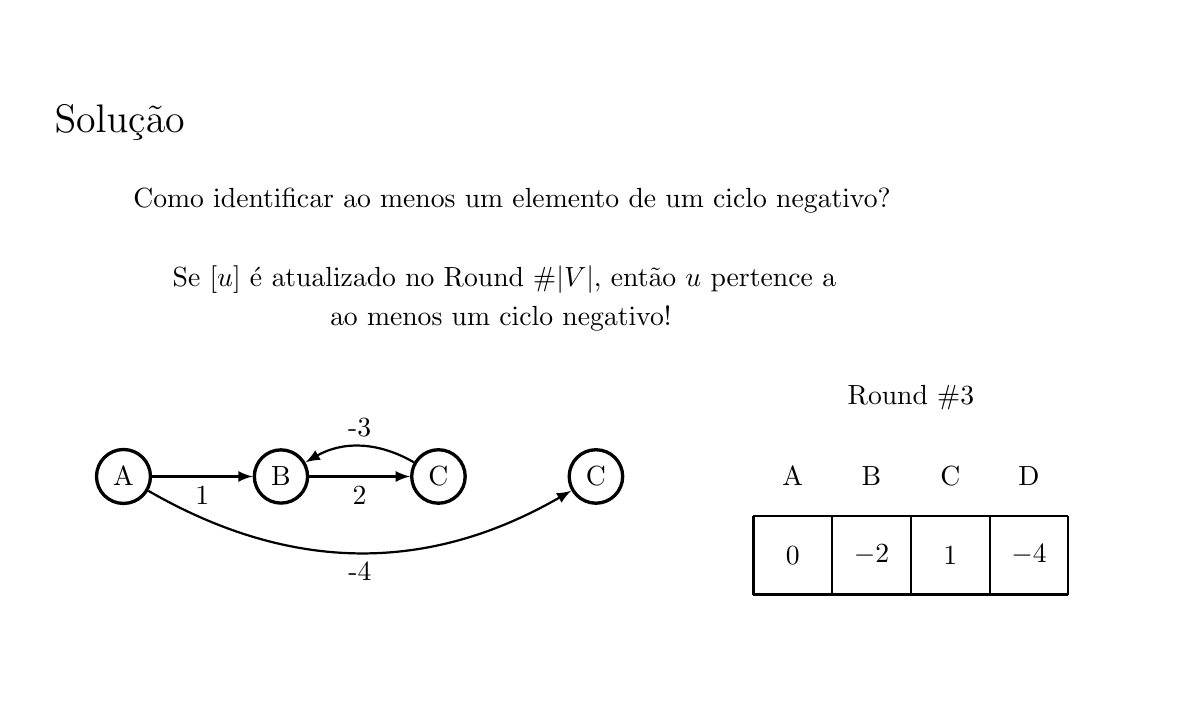
\begin{tikzpicture}
\node[draw,opacity=0] at (0, 0) {x};
\node[draw,opacity=0] at (14, 8) {x};
 \node[anchor=west] at (0, 7) { \Large \bbbold{Solução} };
 \node[anchor=west] at (1, 6) { \bbtext{Como identificar ao menos um elemento de um ciclo negativo? } };
 \node[anchor=west] at (1.5, 5) { \bbcomment{Se $\dist[u]$ é atualizado no Round \#$|V|$, então $u$ pertence a } };
 \node[anchor=west] at (3.5, 4.5) { \bbcomment{ao menos um ciclo negativo! } };
 \node[draw,very thick,circle] (A) at (1, 2.5) { \bbtext{A} };
 \node[draw,very thick,circle] (B) at (3, 2.5) { \bbtext{B} };
 \node[draw,very thick,circle] (C) at (5, 2.5) { \bbtext{C} };
 \node[draw,very thick,circle] (D) at (7, 2.5) { \bbtext{C} };
 \draw[-latex,thick] (A) to node[below] { \bbinfo{1} } (B);
 \draw[-latex,thick] (B) to node[below] { \bbinfo{2} } (C);
 \draw[-latex,thick] (C) to [bend right] node[above] { \bbinfo{-3} } (B);
 \draw[-latex,thick] (A) to [bend right] node[below] { \bbinfo{-4} } (D);
 \draw[thick] (9, 1) grid (13, 2);
 \node at (9.5, 2.5) { \bbtext{A} };
 \node at (10.5, 2.5) { \bbtext{B} };
 \node at (11.5, 2.5) { \bbtext{C} };
 \node at (12.5, 2.5) { \bbtext{D} };
 \node at (9.5, 1.5) { $0$ };
 \node at (12.5, 1.5) { $-4$ };
 \node at (11, 3.5) { \bbbold{Round \#3} };
 \node at (10.5, 1.5) { $-2$ };
 \node at (11.5, 1.5) { $1$ };
\end{tikzpicture}
\end{frame}

\begin{frame}[plain,t]
\begin{tikzpicture}
\node[draw,opacity=0] at (0, 0) {x};
\node[draw,opacity=0] at (14, 8) {x};
 \node[anchor=west] at (0, 7) { \Large \bbbold{Solução} };
 \node[anchor=west] at (1, 6) { \bbtext{Como identificar ao menos um elemento de um ciclo negativo? } };
 \node[anchor=west] at (1.5, 5) { \bbcomment{Se $\dist[u]$ é atualizado no Round \#$|V|$, então $u$ pertence a } };
 \node[anchor=west] at (3.5, 4.5) { \bbcomment{ao menos um ciclo negativo! } };
 \node[draw,very thick,circle] (A) at (1, 2.5) { \bbtext{A} };
 \node[draw,very thick,circle] (D) at (7, 2.5) { \bbtext{C} };
 \draw[-latex,thick] (A) to node[below] { \bbinfo{1} } (B);
 \draw[-latex,thick] (B) to node[below] { \bbinfo{2} } (C);
 \draw[-latex,thick] (C) to [bend right] node[above] { \bbinfo{-3} } (B);
 \draw[-latex,thick] (A) to [bend right] node[below] { \bbinfo{-4} } (D);
 \draw[thick] (9, 1) grid (13, 2);
 \node at (9.5, 2.5) { \bbtext{A} };
 \node at (10.5, 2.5) { \bbtext{B} };
 \node at (11.5, 2.5) { \bbtext{C} };
 \node at (12.5, 2.5) { \bbtext{D} };
 \node at (9.5, 1.5) { $0$ };
 \node at (12.5, 1.5) { $-4$ };
 \node at (11, 3.5) { \bbbold{Round \#4} };
 \node at (10.5, 1.5) { $\mathbf{-3}$ };
 \node at (11.5, 1.5) { $\mathbf{0}$ };
 \node[draw,very thick,circle,fill=BBCyan] (B) at (3, 2.5) { \bbtext{B} };
 \node[draw,very thick,circle,fill=BBCyan] (C) at (5, 2.5) { \bbtext{C} };
\end{tikzpicture}
\end{frame}

\begin{frame}[plain,t]
\begin{tikzpicture}
\node[draw,opacity=0] at (0, 0) {x};
\node[draw,opacity=0] at (14, 8) {x};
 \node[anchor=west] at (0, 7) { \Large \bbbold{Solução} };
\end{tikzpicture}
\end{frame}

\begin{frame}[plain,t]
\begin{tikzpicture}
\node[draw,opacity=0] at (0, 0) {x};
\node[draw,opacity=0] at (14, 8) {x};
 \node[anchor=west] at (0, 7) { \Large \bbbold{Solução} };
 \node[anchor=west] at (1, 6) { \bbtext{Em que casos a pontuação pode ser arbitrariamente grande?} };
\end{tikzpicture}
\end{frame}

\begin{frame}[plain,t]
\begin{tikzpicture}
\node[draw,opacity=0] at (0, 0) {x};
\node[draw,opacity=0] at (14, 8) {x};
 \node[anchor=west] at (0, 7) { \Large \bbbold{Solução} };
 \node[anchor=west] at (1, 6) { \bbtext{Em que casos a pontuação pode ser arbitrariamente grande?} };
 \node[anchor=west] at (1.5, 5) { \bbcomment{Quando há um caminho de um nó de um ciclo negativo até $N$! } };
\end{tikzpicture}
\end{frame}

\begin{frame}[plain,t]
\begin{tikzpicture}
\node[draw,opacity=0] at (0, 0) {x};
\node[draw,opacity=0] at (14, 8) {x};
 \node[anchor=west] at (0, 7) { \Large \bbbold{Solução} };
 \node[anchor=west] at (1, 6) { \bbtext{Em que casos a pontuação pode ser arbitrariamente grande?} };
 \node[anchor=west] at (1.5, 5) { \bbcomment{Quando há um caminho de um nó de um ciclo negativo até $N$! } };
 \node[anchor=west] at (1, 3) { \bbtext{E como posso identificar a existência ou não de tais caminhos? } };
\end{tikzpicture}
\end{frame}

\begin{frame}[plain,t]
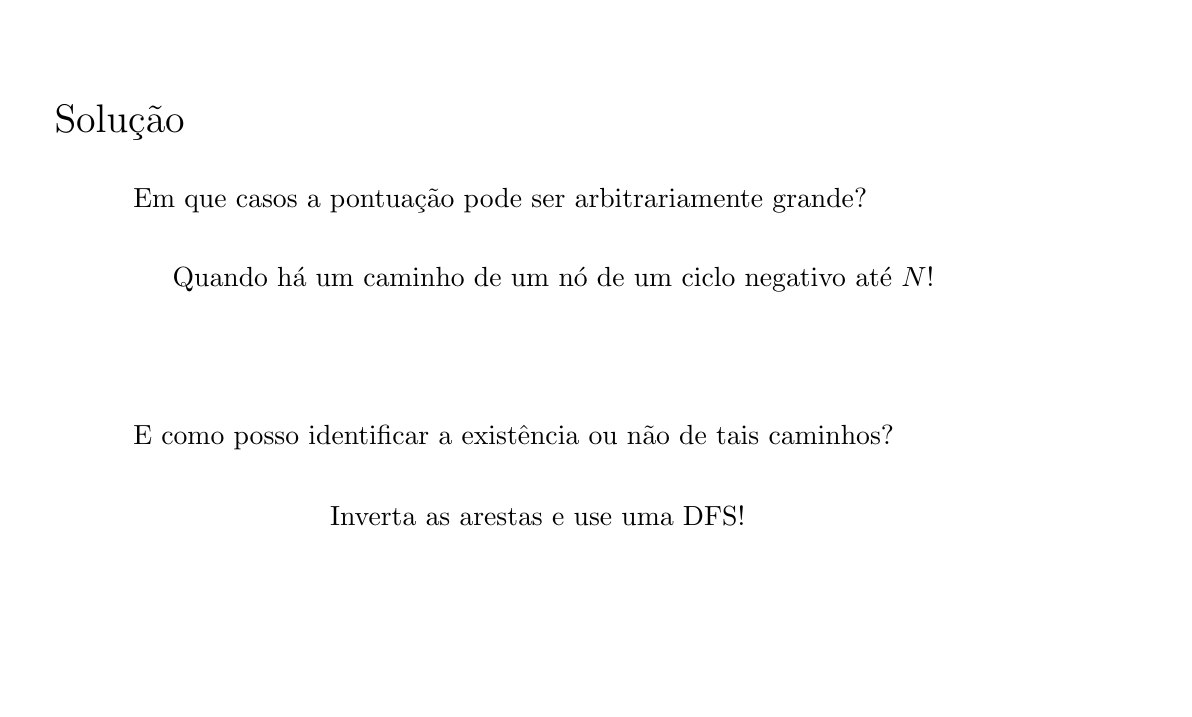
\begin{tikzpicture}
\node[draw,opacity=0] at (0, 0) {x};
\node[draw,opacity=0] at (14, 8) {x};
 \node[anchor=west] at (0, 7) { \Large \bbbold{Solução} };
 \node[anchor=west] at (1, 6) { \bbtext{Em que casos a pontuação pode ser arbitrariamente grande?} };
 \node[anchor=west] at (1.5, 5) { \bbcomment{Quando há um caminho de um nó de um ciclo negativo até $N$! } };
 \node[anchor=west] at (1, 3) { \bbtext{E como posso identificar a existência ou não de tais caminhos? } };
 \node[anchor=west] at (3.5, 2) { \bbcomment{Inverta as arestas e use uma DFS! } };
\end{tikzpicture}
\end{frame}

\begin{frame}[plain,t]
\begin{tikzpicture}
\node[draw,opacity=0] at (0, 0) {x};
\node[draw,opacity=0] at (14, 8) {x};
 \node[draw,very thick,circle] (A) at (3, 7) { \bbtext{A} };
 \node[draw,very thick,circle,fill=BBCyan] (B) at (5, 5) { \bbtext{B} };
 \node[draw,very thick,circle,fill=BBCyan] (C) at (5, 3) { \bbtext{C} };
 \node[draw,very thick,circle] (D) at (1, 5) { \bbtext{D} };
 \draw[-latex,thick] (A) to node[above right] { \bbinfo{3} } (B);
 \draw[-latex,thick] (A) to node[above left] { \bbinfo{2} } (D);
 \draw[-latex,thick] (B) to [bend left] node[right] { \bbinfo{3} } (C);
 \draw[latex-,thick] (B) to [bend right] node[left] { \bbinfo{-5} } (C);
\end{tikzpicture}
\end{frame}

\begin{frame}[plain,t]
\begin{tikzpicture}
\node[draw,opacity=0] at (0, 0) {x};
\node[draw,opacity=0] at (14, 8) {x};
 \node[draw,very thick,circle] (A) at (3, 7) { \bbtext{A} };
 \node[draw,very thick,circle,fill=BBCyan] (B) at (5, 5) { \bbtext{B} };
 \node[draw,very thick,circle,fill=BBCyan] (C) at (5, 3) { \bbtext{C} };
 \node[draw,very thick,circle] (D) at (1, 5) { \bbtext{D} };
 \draw[-latex,thick] (A) to node[above right] { \bbinfo{3} } (B);
 \draw[-latex,thick] (A) to node[above left] { \bbinfo{2} } (D);
 \draw[-latex,thick] (B) to [bend left] node[right] { \bbinfo{3} } (C);
 \draw[latex-,thick] (B) to [bend right] node[left] { \bbinfo{-5} } (C);
 \node at (3, 1.5) { \bbbold{Solução:} \bbtext{2} };
\end{tikzpicture}
\end{frame}

\begin{frame}[plain,t]
\begin{tikzpicture}
\node[draw,opacity=0] at (0, 0) {x};
\node[draw,opacity=0] at (14, 8) {x};
 \node[draw,very thick,circle] (A) at (3, 7) { \bbtext{A} };
 \node[draw,very thick,circle,fill=BBCyan] (B) at (5, 5) { \bbtext{B} };
 \node[draw,very thick,circle,fill=BBCyan] (C) at (5, 3) { \bbtext{C} };
 \node[draw,very thick,circle] (D) at (1, 5) { \bbtext{D} };
 \draw[-latex,thick] (A) to node[above right] { \bbinfo{3} } (B);
 \draw[-latex,thick] (A) to node[above left] { \bbinfo{2} } (D);
 \draw[-latex,thick] (B) to [bend left] node[right] { \bbinfo{3} } (C);
 \draw[latex-,thick] (B) to [bend right] node[left] { \bbinfo{-5} } (C);
 \node at (3, 1.5) { \bbbold{Solução:} \bbtext{2} };
 \node[draw,very thick,circle] (A1) at (10, 7) { \bbtext{A} };
 \node[draw,very thick,circle,fill=BBCyan] (B1) at (12, 5) { \bbtext{B} };
 \node[draw,very thick,circle,fill=BBCyan] (C1) at (12, 3) { \bbtext{C} };
 \node[draw,very thick,circle] (D1) at (8, 5) { \bbtext{D} };
 \draw[-latex,thick] (A1) to [bend left] node[above right] { \bbinfo{3} } (B1);
 \draw[latex-,thick] (A1) to [bend right] node[below left] { \bbinfo{1} } (B1);
 \draw[-latex,thick] (A1) to node[above left] { \bbinfo{2} } (D1);
 \draw[-latex,thick] (B1) to [bend left] node[right] { \bbinfo{3} } (C1);
 \draw[latex-,thick] (B1) to [bend right] node[left] { \bbinfo{-5} } (C1);
\end{tikzpicture}
\end{frame}

\begin{frame}[plain,t]
\begin{tikzpicture}
\node[draw,opacity=0] at (0, 0) {x};
\node[draw,opacity=0] at (14, 8) {x};
 \node[draw,very thick,circle] (A) at (3, 7) { \bbtext{A} };
 \node[draw,very thick,circle,fill=BBCyan] (B) at (5, 5) { \bbtext{B} };
 \node[draw,very thick,circle,fill=BBCyan] (C) at (5, 3) { \bbtext{C} };
 \node[draw,very thick,circle] (D) at (1, 5) { \bbtext{D} };
 \draw[-latex,thick] (A) to node[above right] { \bbinfo{3} } (B);
 \draw[-latex,thick] (A) to node[above left] { \bbinfo{2} } (D);
 \draw[-latex,thick] (B) to [bend left] node[right] { \bbinfo{3} } (C);
 \draw[latex-,thick] (B) to [bend right] node[left] { \bbinfo{-5} } (C);
 \node at (3, 1.5) { \bbbold{Solução:} \bbtext{2} };
 \node[draw,very thick,circle] (A1) at (10, 7) { \bbtext{A} };
 \node[draw,very thick,circle,fill=BBCyan] (B1) at (12, 5) { \bbtext{B} };
 \node[draw,very thick,circle,fill=BBCyan] (C1) at (12, 3) { \bbtext{C} };
 \node[draw,very thick,circle] (D1) at (8, 5) { \bbtext{D} };
 \draw[-latex,thick] (A1) to [bend left] node[above right] { \bbinfo{3} } (B1);
 \draw[latex-,thick] (A1) to [bend right] node[below left] { \bbinfo{1} } (B1);
 \draw[-latex,thick] (A1) to node[above left] { \bbinfo{2} } (D1);
 \draw[-latex,thick] (B1) to [bend left] node[right] { \bbinfo{3} } (C1);
 \draw[latex-,thick] (B1) to [bend right] node[left] { \bbinfo{-5} } (C1);
 \node at (10, 1.5) { \bbbold{Solução:} \bbalert{-1} };
\end{tikzpicture}
\end{frame}

\begin{frame}[plain,t]
 \inputsnippet{cpp}{31}{50}{codes/1673.cpp}
\end{frame}

\begin{frame}[plain,t]
 \inputsnippet{cpp}{14}{29}{codes/1673.cpp}
\end{frame}

\end{document}
